% Graphical abstract concept 3: the stream replaces the generation.
% Left: generation-staged ABC-SMC, populations that must fill before the next
% proposal forms. Right: the single-arrival stream, a top-k archive, a proposal
% rebuilt after every arrival, and every particle weighted against the mixture
% of proposals actually used.
\documentclass[tikz,border=4pt]{standalone}
\usepackage{newtxtext,newtxmath}
\usetikzlibrary{arrows.meta,decorations.pathreplacing,calc,positioning}
\definecolor{async}{HTML}{0072B2}
\definecolor{sync}{HTML}{D55E00}
\definecolor{reject}{HTML}{009E73}

\begin{document}
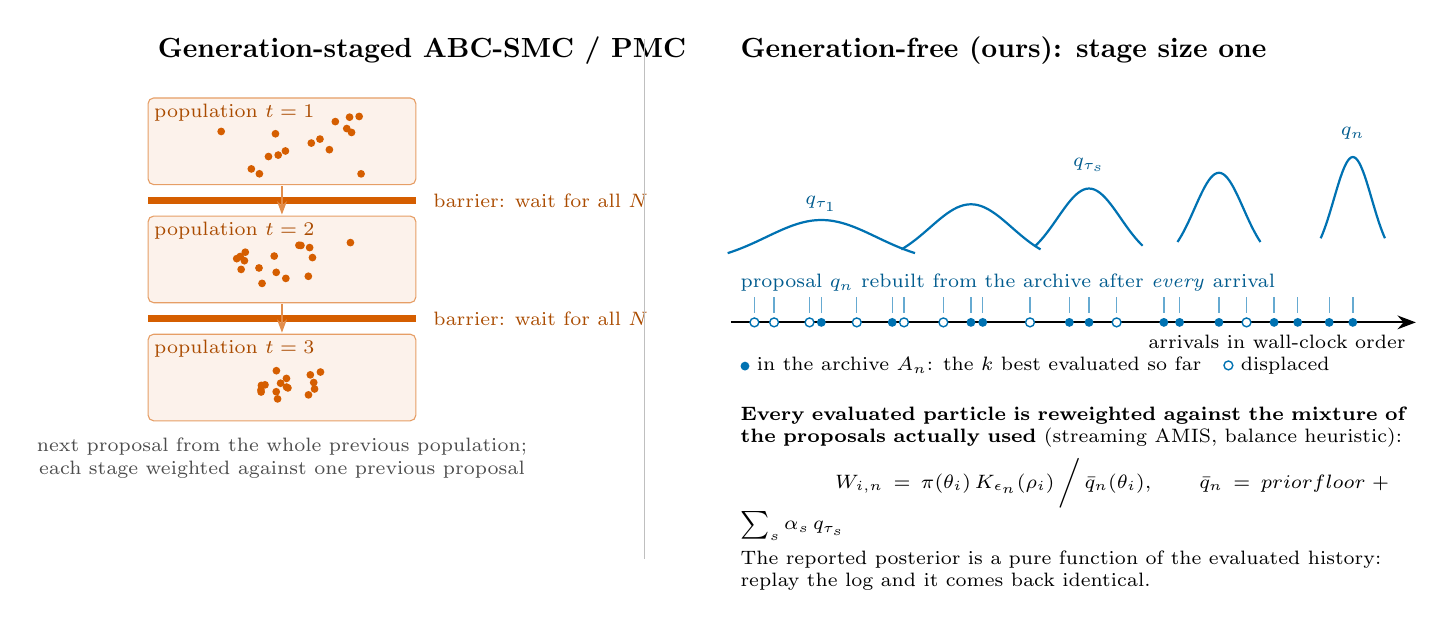
\begin{tikzpicture}[font=\small,>=Stealth]

%% ------------------------------------------------------- left: generations
\node[font=\bfseries,anchor=west] at (0,3.45) {Generation-staged ABC-SMC / PMC};
\foreach \g/\y/\sx/\sy in {1/2.3/1.15/0.42, 2/0.8/0.75/0.30, 3/-0.7/0.42/0.20} {
  \draw[rounded corners=2pt,fill=sync!8,draw=sync!60] (0,\y-0.55) rectangle (3.4,\y+0.55);
  \node[anchor=north west,font=\scriptsize,text=sync!80!black,inner sep=2pt] at (0,\y+0.55) {population $t=\g$};
  \pgfmathsetseed{20+\g}
  \foreach \i in {1,...,16} {
    \pgfmathsetmacro{\px}{1.85+\sx*rand}
    \pgfmathsetmacro{\py}{\y-0.08+\sy*rand}
    \fill[sync] (\px,\py) circle (1.4pt);
  }
}
\foreach \y in {1.55,0.05} {
  \draw[sync,line width=2.6pt] (0,\y) -- (3.4,\y);
  \node[anchor=west,font=\scriptsize,text=sync!80!black] at (3.5,\y) {barrier: wait for all $N$};
  \draw[->,sync!70] (1.7,\y+0.18) -- (1.7,\y-0.18);
}
\node[anchor=north,font=\scriptsize,align=center,text=black!70] at (1.7,-1.35)
  {next proposal from the whole previous population;\\each stage weighted against one previous proposal};

%% ------------------------------------------------------- right: the stream
\begin{scope}[shift={(7.4,0)}]
\node[font=\bfseries,anchor=west] at (0,3.45) {Generation-free (ours): stage size one};
% time axis with arrivals; filled = currently in the top-k archive
\draw[->,thick] (0,0) -- (8.7,0) node[below left,font=\scriptsize,yshift=-1pt] {arrivals in wall-clock order};
\foreach \x/\inarch in {0.3/0,0.55/0,1.0/0,1.15/1,1.6/0,2.05/1,2.2/0,2.7/0,3.05/1,3.2/1,3.8/0,4.3/1,4.55/1,4.9/0,5.5/1,5.7/1,6.2/1,6.55/0,6.9/1,7.2/1,7.6/1,7.9/1} {
  \ifnum\inarch=1
    \fill[async] (\x,0) circle (1.6pt);
  \else
    \draw[async,fill=white,line width=0.5pt] (\x,0) circle (1.6pt);
  \fi
}
% a proposal is rebuilt at every arrival: one tick each
\foreach \x in {0.3,0.55,1.0,1.15,1.6,2.05,2.2,2.7,3.05,3.2,3.8,4.3,4.55,4.9,5.5,5.7,6.2,6.55,6.9,7.2,7.6,7.9} {
  \draw[async!60,line width=0.5pt] (\x,0.12) -- (\x,0.32);
}
\node[anchor=west,font=\scriptsize,text=async!80!black] at (0,0.5) {proposal $q_n$ rebuilt from the archive after \emph{every} arrival};
% five of the proposals drawn, narrowing as the tolerance tightens
\foreach \x/\w/\h in {1.15/0.70/0.55, 3.05/0.52/0.75, 4.55/0.40/0.95, 6.2/0.31/1.15, 7.9/0.24/1.35} {
  \draw[async,line width=0.8pt,domain=-1.7:1.7,variable=\t,samples=41,smooth]
    plot ({\x+\w*\t},{0.75+\h*exp(-0.5*\t*\t)});
}
\node[font=\scriptsize,text=async!80!black] at (1.15,1.5) {$q_{\tau_1}$};
\node[font=\scriptsize,text=async!80!black] at (4.55,2.0) {$q_{\tau_s}$};
\node[font=\scriptsize,text=async!80!black] at (7.9,2.4) {$q_n$};
% archive legend
\node[anchor=west,font=\scriptsize,align=left] at (0,-0.55)
  {\tikz\fill[async] (0,0) circle (1.6pt); in the archive $A_n$: the $k$ best evaluated so far\quad
   \tikz\draw[async,fill=white,line width=0.5pt] (0,0) circle (1.6pt); displaced};
% the reported estimator: weight against the mixture of all proposals used
\node[anchor=north west,font=\scriptsize,align=left,text width=8.6cm] at (0,-0.95)
  {\textbf{Every evaluated particle is reweighted against the mixture of the proposals actually used}
   (streaming AMIS, balance heuristic):\\[3pt]
   \hspace*{1.2cm}$W_{i,n}=\pi(\theta_i)\,K_{\epsilon_n}(\rho_i)\,\big/\,\bar q_n(\theta_i),\qquad
   \bar q_n=\text{prior floor}+\textstyle\sum_{s}\alpha_{s}\,q_{\tau_s}$\\[3pt]
   The reported posterior is a pure function of the evaluated history: replay the log and it comes back identical.};
\end{scope}

%% ------------------------------------------------------- divider
\draw[black!25] (6.3,3.6) -- (6.3,-3.0);
\end{tikzpicture}
\end{document}
